%%%%%%%%%%%%%%
% Homework 8 %
%%%%%%%%%%%%%%

\documentclass[letter]{article}

\usepackage[pdftex]{graphicx}
\usepackage[margin=1.25in]{geometry}
\usepackage[english]{babel}
\usepackage{listings}
\usepackage{amsthm}
\usepackage{amssymb}
\usepackage{framed} 
\usepackage{amsmath, mathtools}
\usepackage{pgfplots}
\usepackage{titling}
\usepackage{fancyhdr}
\usepackage{tikz}
\usepackage[american]{circuitikz}

\pagestyle{fancy}

\newtheorem{theorem}{Theorem}[section]

\newenvironment{menumerate}{\edef\backupindent{\the\parindent}
  \enumerate\setlength{\parindent}{\backupindent}}
  {\endenumerate}

\lstset{language=python}

\pgfplotsset{compat=1.13}

%%%%%%%%%%%%%%
%  Doc Info  %
%%%%%%%%%%%%%%
\newcommand{\hwn}{8}
\newcommand{\class}{EE 16A}

\title{\class: Homework \hwn}
\author{David J. Lee\\3031796951\\dssd1001@berkeley.edu}

\fancyhead[L]{\class}
\fancyhead[C]{Homework \hwn}
\fancyhead[R]{\thepage}
\fancyfoot{}

%%%%%%%%%%%%%%

\begin{document}
\maketitle
\thispagestyle{empty}

\begin{menumerate}
    \item \textbf{Worked With...}
    
    Ilya (3031806896), James Zhu (3031793129)\\
    I worked alone on Friday morning, then met up with Ilya and James to discuss on Saturday afternoon.
    
    \newpage
    \item \textbf{Basic Amplifier Building Blocks}
    \begin{center}
        \includegraphics[scale=0.2]{q2diag.png}
    \end{center}
    \begin{menumerate}
        \item \emph{Label the input terminals of the Op-amp so it is in negative feedback. Then, derive the voltage gain of the non-inverting amplifier using the Golden Rules. Explain the origin of the name of the amplifier.}
        \begin{center}
            \includegraphics[scale=0.2]{2blabel2.png}
        \end{center}
        From the Golden Rules, we know that
        \begin{equation*}
            \begin{split}
                I_+ &= I_\_ = 0\\
                V_+ &= V_\_\\
                V_+ &= v_s
            \end{split}
        \end{equation*}
        Thus we can reduce the bottom half circuit to a simple voltage divider to get
        \begin{center}
        \begin{circuitikz}
            \draw (0,0) node[ground]{}
                to [R=$R_1$] ++(2,0)
                to [R=$R_2$,-o] ++(2,0) node[right]{$v_0$};
            \draw (0,0) to [short,*-o] ++(0,1);
            \draw (2,0) to [short,*-o] ++(0,1);
            \draw (0.75,1) node[right] {$V_\_$};
        \end{circuitikz}
        \end{center}
        \begin{equation*}
            V_\_ = v_s = \frac{R_1}{R_1 + R_2} v_o\\
        \end{equation*}
        which gives the voltage gain of
        \begin{equation*}
            \boxed{\frac{v_o}{v_s} = 1 + \frac{R_2}{R_1}}
        \end{equation*}
        Name makes sense from the fact that the gain is non-negative and $>$1.
        
        \item \emph{Label the input terminals of the Op-amp so it is negative feedback. Then, derive the voltage gain of the inverting amplifier using the Golden Rules. Explain the origin of the name of the amplifier.}
        \begin{center}
            \includegraphics[scale=0.2]{2blabel.png}
        \end{center}
        First, we use the Golden Rules, and the fact that the opamp is connected in negative feedback, to get
        \begin{equation*}
            V_\_ = V_+ = 0
        \end{equation*}
        Also, since we know that the current through each terminal of the opamp will be 0 (fromt the Golden Rules), we can write the following nodal analysis equation at the - terminal of the opamp:
        \begin{equation*}
            \frac{v_s - V_\_}{R_1} = \frac{V_\_ - v_o}{R_2}
        \end{equation*}
        which gives the voltage gain of
        \begin{equation*}
            \boxed{\frac{v_o}{v_s} = -\frac{R_2}{R_1}}
        \end{equation*}
        Name makes sense from the fact that the gain is negative.
    \end{menumerate}
    
    \newpage
    \item \textbf{Amplifier with Multiple Inputs}
    \begin{center}
        \includegraphics[scale=0.2]{q3diag.png}
    \end{center}
    \begin{menumerate}
        \item \emph{Use the Golden Rules to find $v_{o2}$ for the first circuit.}
        \begin{equation*}
            V_\_ = V_+ = 0
        \end{equation*}
        Conduct nodal analysis at the - terminal of the opamp:
        \begin{equation*}
            \begin{split}
                \frac{0 - 0}{R_1} + \frac{0 - v_{o2}}{R_2} + i_{s3} = 0\\
                -\frac{v_{o2}}{R_2} + i{s3} = 0\\
                \boxed{v_{o2} = R_2i_{s3}}
            \end{split}
        \end{equation*}
        \item \emph{Use the Golden Rules to find $v_{o3}$ for the second circuit.}
        \begin{equation*}
            V_\_ = V_+ = v_{s2}
        \end{equation*}
        Nodal analysis at the - terminal of the opamp:
        \begin{equation*}
            \begin{split}
                \frac{v_{s2} - 0}{R_1} + \frac{v_{s2} - v_{o3}}{R_2} = 0\\
                -\frac{R_2}{R_1} = \frac{-v_{s2} + v_{o3}}{v_{s2}}\\
                \boxed{v_{o3} = v_{s2}(1 + \frac{R_2}{R_1})}
            \end{split}
        \end{equation*}
        \item \emph{Use the Golden Rules to find the output voltage $v_o$ for the circuit.}
        \begin{center}
            \includegraphics[scale=0.2]{q3cdiag.png}
        \end{center}
        \begin{equation*}
            V_\_ = V_+ = v_{s2}
        \end{equation*}
        Nodal analysis at the - terminal of the opamp:
        \begin{equation*}
            \begin{split}
                \frac{v_{s2} - v_{s1}}{R_1} + \frac{v_{s2} - v_o}{R_2} + i_{s3} = 0\\
                i_{s3} + \frac{v_{s2} - v_{s1}}{R_1} = \frac{v_o - v_{s2}}{R_2}
            \end{split}
        \end{equation*}
        \begin{equation}
            \boxed{v_o = R_2i_{s3} + \frac{R_2}{R_1}(v_{s2} - v_{s1}) + v_{s2}}
        \end{equation}
        \item \emph{Now add a second stage. What is $v_{o, new}$? Does $v_o$ change between the last part and this part? Does the voltage $v_{o, new}$ depend on $R_L$?}
        \begin{center}
            \includegraphics[scale=0.2]{q3ddiag.png}
        \end{center}
        \begin{equation*}
            V_\_ = V_+ = v_o
        \end{equation*}
        Nodal analysis at the - terminal of the opamp:
        \begin{equation*}
            \begin{split}
                \frac{v_o - 0}{R_4} + \frac{v_o - v_{o,new}}{R_3} = 0\\
                v_{o,new} = v_o(1 + \frac{R_3}{R_4})
            \end{split}
        \end{equation*}
        where $v_o$ stays the same ($R_2i_{s3} + \frac{R_2}{R_1}(v_{s2} - v_{s1}) + v_{s2}$) from equation (1), and thus
        \begin{equation*}
            \boxed{v_{o,new} = (1 + \frac{R_3}{R_4})(R_2i_{s3} + \frac{R_2}{R_1}(v_{s2} - v_{s1}) + v_{s2})}
        \end{equation*}
        We can also see that $v_{o,new}$ does not depend on $R_L$.
    \end{menumerate}
    
    \newpage
    \item \textbf{It's finally raining!} \emph{A lettuce farmer in the Salinas valley has grown tired of weather.com?s imprecise rain measurements. So, she decided to take matters into her own hands by building a rain sensor. She placed a rectangular tank outside and attached two metal plates to two opposite sides in an effort to make a capacitor whose capacitance varies with the amount of water inside.\\The width and length of the tank are both $w$ (i.e. the base is square) and the height of the tank is $h_{tot}$.}
    \begin{center}
        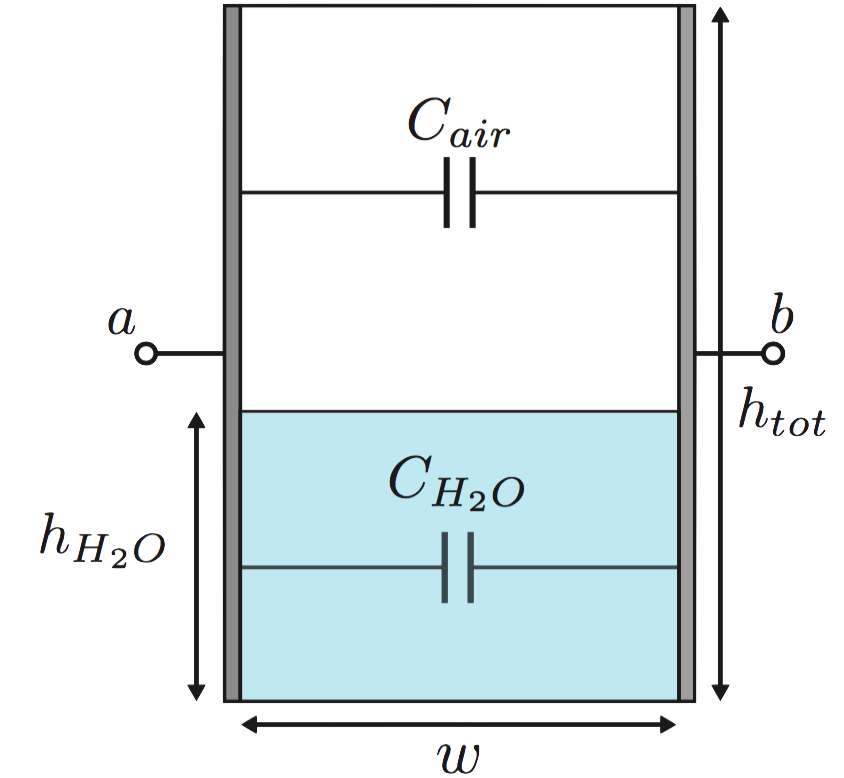
\includegraphics[scale=0.15]{q4diag.png}
    \end{center}
    \begin{menumerate}
        \item \emph{What is the capacitance between terminals $a$ and $b$ when the tank is full? What about when it is empty?}
        
        Full:
            $81\epsilon\cdot \frac{w\cdot h_{tot}}{w} = \boxed{81\epsilon h_{tot}}$
            
        Empty:
            $\boxed{\epsilon h_{tot}}$
        \item \emph{Suppose the heightofthewaterinthetankis $h_{H_2O}$. Modeling the tankasapairofcapacitors inparallel, find the total capacitance between the two plates, $C_{tank}$.}
            \begin{equation*}
            \begin{split}
                C_{air} &= \epsilon\frac{w\cdot(h_{tot}-h_{H_2O})}{w}\\
                &= \epsilon(h_{tot}-h_{H_2O})\\
                C_{H_2O} &= 81\epsilon\frac{w\cdot h_{H_2O}}{w}\\
                &= 81\epsilon h_{H_2O}\\
                C_{tank} = C_{air} + C_{H_2O} &= \boxed{\epsilon(80h_{H_2O}+h_{tot})}
            \end{split}
            \end{equation*}
        \item \emph{Find the voltage $V_o$ in phase $\Phi_2$ as a function of the height of the water.}
        \begin{center}
            \includegraphics[scale=0.2]{q4cdiag.png}
        \end{center}
        \begin{center} \textbf{Phase 1:}
        \begin{center} \begin{circuitikz}
            \draw node[ground]{} to [V, v=$V_{in}$] (2,0)
            to [C=$C_{tank}$] ++ (0,-1)
            to [C=$C_{known}$] ++ (0,-1)node[ground]{};
        \end{circuitikz} \end{center}
        where the charge on each place is
        \begin{equation}
            Q = (C_{tank}||C_{known})\cdot V_{in}
        \end{equation}
        \textbf{Phase 2:}
        \begin{center} \begin{circuitikz}
            \draw (0,0)node[ground]{} to [C=$C_{known}$] ++ (0,1)
            to [short, -o] ++ (3,0) node[right]{$V_o$};
            \draw (2,0)node[ground]{} to [C=$C_{tank}$] ++ (0,1);
        \end{circuitikz} \end{center}
        $\downarrow$
        \begin{center} \begin{circuitikz}
            \draw (0,0)node[ground]{} to [C=$C_{known}+C_{tank}$] ++ (0,1)
            to [short, -o] ++ (2,0) node[right]{$V_o$};
        \end{circuitikz} \end{center}
        where the charge on the effective plate $C_{known}+C_{tank}$ is $2Q$, thus
        \begin{equation*}
            V_o = \frac{2Q}{C_{known}+C_{tank}}
        \end{equation*}
        and plugging in equation (2) from above, we get
        \begin{equation*}
        \begin{split}
            &= \frac{2V_{in}(C_{known}||C_{tank})}{C_{known}+C_{tank}}\\
            \Aboxed{
            V_o(h_{H_2O}) &= 2V_{in}\frac{C_{known}C_{tank}}{(C_{known}+C_{tank})^2}
            }
        \end{split}
        \end{equation*}
        where $C_{tank} =  \epsilon(80h_{H_2O}+h_{tot})$
        \end{center}
        \item \emph{Plot this voltage $V_o$ as a function of the height of the water. Vary the tank from empty to full. Use values of $V_{in} = 12V, w = 0.5m, h_{tot} = 1m,$ and $\epsilon = 8.854 � 10?12F/m$. For $C_{known}$ use a similar tank that is known to always be empty.}
        
        $V_{in} = 12V$
        
        $ w = 0.5m$
        
        $h_{tot} = 1m$
        
        $\epsilon = 8.854 � 10?12F/m$
        
        $C_{known} = \epsilon h_{tot} = \epsilon$
        \begin{center}
        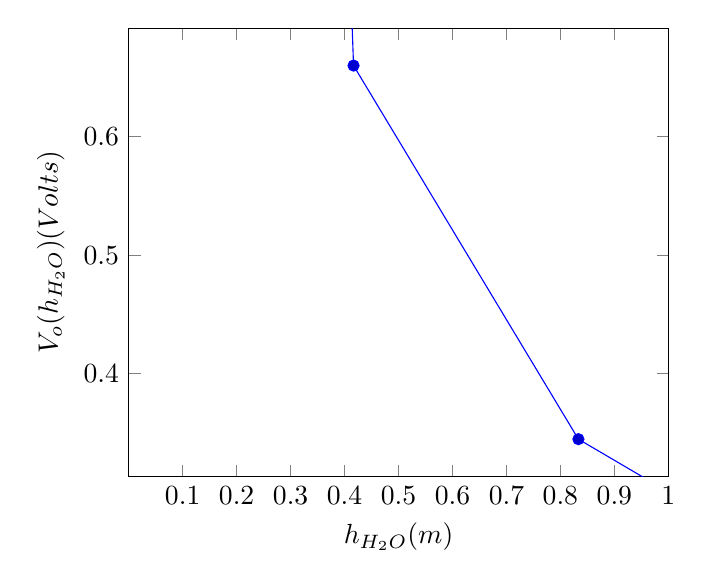
\begin{tikzpicture}
            \begin{axis}[ xlabel=$h_{H_2O} (m)$,
            ylabel={$V_o(h_{H_2O}) (Volts)$},
            xmin=0,xmax=1,xtick={0.1,0.2,...,0.9,1}] 
            \addplot {(1920*x + 24)/(80*x + 2)^2}; 
            \end{axis}
        \end{tikzpicture}
        \end{center}
        \item \emph{What does $V_o$ represent? It?s something we can measure! Our original goal was to determine what the height of the water in the tank without having to look inside it. Rewrite the last part to solve for $h_{water}$.}\\
        $V_o$ represents the output voltage that is measured in a voltmeter or some other device of the lettuce farmer's liking. With that measurement and with some simple rearrangement, the farmer can know what the precise rain measurements are.
        \begin{equation*}
        \begin{split}
            V_o &= 2V_{in}\frac{C_{known}C_{tank}}{(C_{known}+C_{tank})^2}\\
            \frac{V_o}{2V_{in}} &= \frac{C_{known}C_{tank}}{(C_{known}+C_{tank})^2}\\
            \frac{V_o}{2V_{in}}\cdot(C_{known}+C_{tank})^2 &= C_{known}C_{tank}
        \end{split}
        \end{equation*}
        which becomes a messy quadratic in the form $ax^2 + bx + c$
        \begin{equation*}
            \frac{V_o}{2V_{in}}C_{tank}^2 + (\frac{V_o}{V_{in}} - 1)C_{known}C_{tank} + \frac{V_o}{2V_{in}}C_{known}^2 = 0
        \end{equation*}
        Solving for $C_{tank}$, we get
        \begin{equation*}
            \begin{split}
                C_{tank} &= \frac{-b \pm \sqrt{b^2 -4ac}}{2a}\\
                &= \frac{-(\frac{V_o}{V_{in}} - 1)C_{known} + \sqrt{((\frac{V_o}{V_{in}} - 1)C_{known})^2 -(\frac{V_o}{V_{in}}C_{known})^2}}{\frac{V_o}{V_{in}}}\\
                &= \frac{V_{in}}{V_o}C_{known} - C_{known} + C_{known}\sqrt{(\frac{V_{in}}{V_o})^2 - 2\frac{V_{in}}{V_o}}\\
                &= C_{known}(\frac{V_{in}}{V_o} - 1 + \sqrt{(\frac{V_{in}}{V_o})^2 - 2\frac{V_{in}}{V_o}})
            \end{split}
        \end{equation*}
        And knowing that $C_{tank} = \epsilon(80h_{H_2O} + h_{tot})$, we solve for $h_{H_2O}$ to get
        \begin{equation*}
            \boxed{h_{H_2O} = \frac{C_{known}(\frac{V_{in}}{V_o} - 1 + \sqrt{(\frac{V_{in}}{V_o})^2 - 2\frac{V_{in}}{V_o}}) - \epsilon h_{tot}}{80\epsilon}}
        \end{equation*}
        \item \emph{What are the units of your result for $V_o$ and for $h_{water}$?}
        
        For $V_o$:
        \begin{equation*}
            V_o(h_{H_2O}) = 2V_{in}\frac{C_{known}C_{tank}}{(C_{known}+C_{tank})^2}
        \end{equation*}
        Capacitances cancel out to give us a unit of \boxed{Volts}.
               
        For $h_{water}$:
        \begin{equation*}
            h_{H_2O} = \frac{C_{known}(\frac{V_{in}}{V_o} - 1 + \sqrt{1 - 2\frac{V_o}{V_{in}}}) - \epsilon h_{tot}}{80\epsilon}
        \end{equation*}
        The numerator is in Farads, the denominator $\epsilon$ is in $\frac{F}{m}$, giving us a unit of \boxed{meters}.
    \end{menumerate}
    

\end{menumerate}

\end{document}
